\subsectionold{x86}

\subsubsectionold{x86 + MSVC}

Here is how the \TT{f\_signed()} function looks like:

\lstinputlisting[caption=\NonOptimizing MSVC 2010]{patterns/07_jcc/simple/signed_MSVC.asm}

\myindex{x86!\Instructions!JLE}

The first instruction, \JLE, stands for \IT{Jump if Less or Equal}. 
In other words, if the second operand is 
larger or equal to the first one, the control flow will be passed to the specified in the instruction address or label.
If this condition does not trigger because the second operand is smaller than the first one, the control flow would not be altered and the first \printf would be executed.
\myindex{x86!\Instructions!JNE}
The second check is \JNE: \IT{Jump if Not Equal}.
The control flow will not change if the operands are equal.

\myindex{x86!\Instructions!JGE}
The third check is \JGE: \IT{Jump if Greater or Equal}---jump if the first operand is larger than 
the second or if they are equal.
So, if all three conditional jumps are triggered, none of the \printf calls would be executed whatsoever. 
This is impossible without special intervention.
Now let's take a look at the \TT{f\_unsigned()} function.
The \TT{f\_unsigned()} function is the same as \TT{f\_signed()}, with the exception that the \JBE and \JAE instructions
are used instead of \JLE and \JGE, as follows:

\lstinputlisting[caption=GCC]{patterns/07_jcc/simple/unsigned_MSVC.asm}

\myindex{x86!\Instructions!JBE}
\myindex{x86!\Instructions!JAE}

As already mentioned, the branch instructions are different:
\JBE---\IT{Jump if Below or Equal} and \JAE\EMDASH{}\IT{Jump if Above or Equal}.
These instructions (\JA/\JAE/\JB/\JBE) differ from \JG/\JGE/\JL/\JLE in the fact that they work with unsigned numbers.

\myindex{x86!\Instructions!JA}
\myindex{x86!\Instructions!JB}
\myindex{x86!\Instructions!JG}
\myindex{x86!\Instructions!JL}
\myindex{Signed numbers}

See also the section about signed number representations~(\myref{sec:signednumbers}).
That is why if we see \JG/\JL in use instead of \JA/\JB or vice-versa, 
we can be almost sure that the variables are signed or unsigned, respectively.
Here is also the \main function, where there is nothing much new to us:

\lstinputlisting[caption=\main]{patterns/07_jcc/simple/main_MSVC.asm}

\clearpage
\subsubsection{x86 + MSVC + \olly}
\myindex{\olly}
\myindex{x86!\Registers!\Flags}

We can see how flags are set by running this example in \olly.
Let's begin with \TT{f\_unsigned()}, which works with unsigned numbers.

\CMP is executed thrice here, but for the same arguments, so the flags are the same each time.

Result of the first comparison:

\begin{figure}[H]
\centering
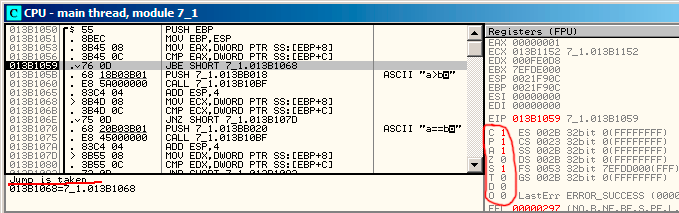
\includegraphics[scale=\FigScale]{patterns/07_jcc/simple/olly_unsigned1.png}
\caption{\olly: \TT{f\_unsigned()}: first conditional jump}
\label{fig:jcc_olly_unsigned_1}
\end{figure}

So, the flags are: C=1, P=1, A=1, Z=0, S=1, T=0, D=0, O=0.

They are named with one character for brevity in \olly.

\olly gives a hint that the (\JBE) jump is to be triggered now.
Indeed, if we take a look into \cite{Intel}, 
we can read there that \JBE is triggering if CF=1 or ZF=1.
The condition is true here, so the jump is triggered.

\clearpage
The next conditional jump:

\begin{figure}[H]
\centering
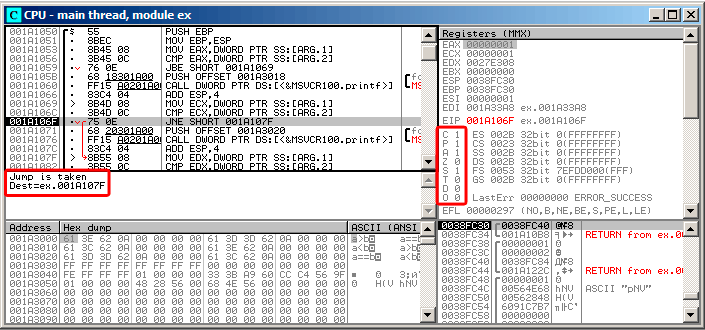
\includegraphics[scale=\FigScale]{patterns/07_jcc/simple/olly_unsigned2.png}
\caption{\olly: \TT{f\_unsigned()}: second conditional jump}
\label{fig:jcc_olly_unsigned_2}
\end{figure}

\olly gives a hint that \JNZ is to be triggered now.
Indeed, \JNZ triggering if ZF=0 (zero flag).

\clearpage
The third conditional jump, \JNB:

\begin{figure}[H]
\centering
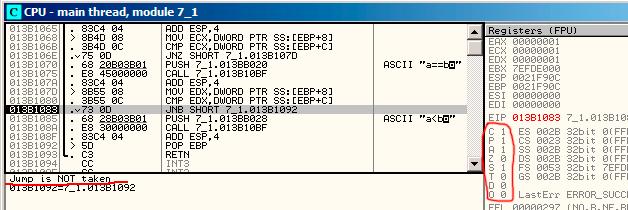
\includegraphics[scale=\FigScale]{patterns/07_jcc/simple/olly_unsigned3.png}
\caption{\olly: \TT{f\_unsigned()}: third conditional jump}
\label{fig:jcc_olly_unsigned_3}
\end{figure}

In \cite{Intel} we can see that \JNB triggers if CF=0 (carry flag).
That is not true in our case, so the third \printf will execute.

\clearpage
Now let's review the \TT{f\_signed()} function, which works with signed values, in \olly.
Flags are set in the same way: C=1, P=1, A=1, Z=0, S=1, T=0, D=0, O=0.
The first conditional jump \JLE is to be triggered:

\begin{figure}[H]
\centering
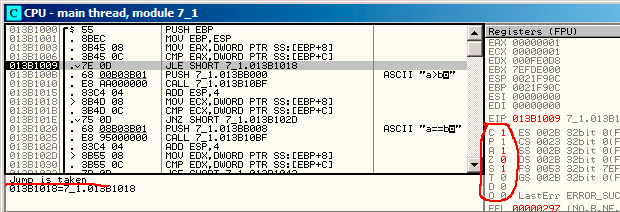
\includegraphics[scale=\FigScale]{patterns/07_jcc/simple/olly_signed1.png}
\caption{\olly: \TT{f\_signed()}: first conditional jump}
\label{fig:jcc_olly_signed_1}
\end{figure}

In \cite{Intel} we find that this instruction is triggered if ZF=1 or SF$\neq$OF.
SF$\neq$OF in our case, so the jump triggers.

\clearpage
The second \JNZ conditional jump triggering: if ZF=0 (zero flag):

\begin{figure}[H]
\centering
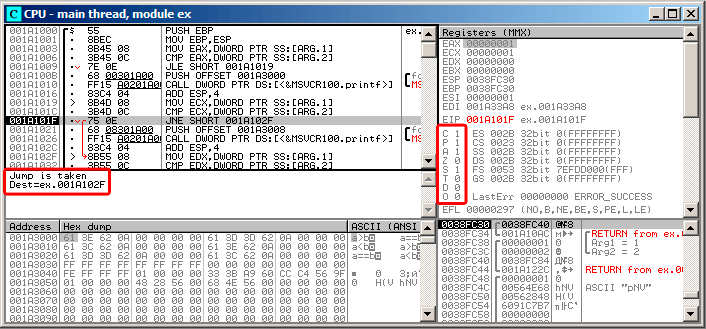
\includegraphics[scale=\FigScale]{patterns/07_jcc/simple/olly_signed2.png}
\caption{\olly: \TT{f\_signed()}: second conditional jump}
\label{fig:jcc_olly_signed_2}
\end{figure}

\clearpage
The third conditional jump \JGE will not trigger because it would only do so if SF=OF, and that is not true in our case:

\begin{figure}[H]
\centering
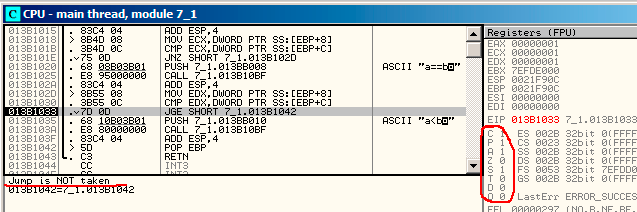
\includegraphics[scale=\FigScale]{patterns/07_jcc/simple/olly_signed3.png}
\caption{\olly: \TT{f\_signed()}: third conditional jump}
\label{fig:jcc_olly_signed_3}
\end{figure}


\clearpage
\subsubsectionold{x86 + MSVC + Hiew}
\myindex{Hiew}

We can try to patch the executable file in a way 
that the \TT{f\_unsigned()} function would always print \q{a==b}, 
no matter the input values.
Here is how it looks in Hiew:

\begin{figure}[H]
\centering
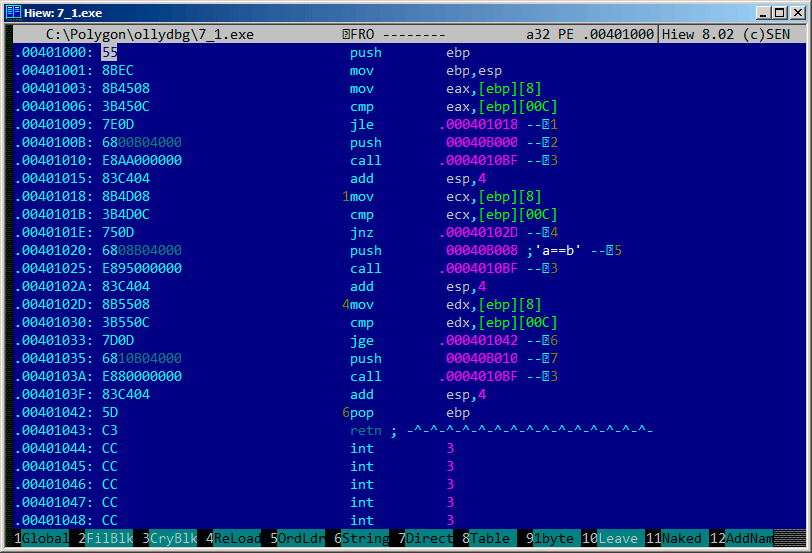
\includegraphics[scale=\FigScale]{patterns/07_jcc/simple/hiew_unsigned1.png}
\caption{Hiew: \TT{f\_unsigned()} function}
\label{fig:jcc_hiew_1}
\end{figure}

Essentially, we need to accomplish three tasks:
\begin{itemize}
\item force the first jump to always trigger;
\item force the second jump to never trigger;
\item force the third jump to always trigger.
\end{itemize}

Thus we can direct the code flow to always pass through the second \printf, and output \q{a==b}.

Three instructions (or bytes) has to be patched:

\begin{itemize}
\item The first jump becomes \JMP, but the \gls{jump offset} would remain the same.

\item 
The second jump might be triggered sometimes, but in any case it will jump to the next
instruction, because, we set the \gls{jump offset} to 0.

In these instructions the \gls{jump offset} is added to the address for the next instruction.
So if the offset is 0,
the jump will transfer the control to the next instruction.

\item 
The third jump we replace with \JMP just as we do with the first one, so it will always trigger.

\end{itemize}

\clearpage
Here is the modified code:

\begin{figure}[H]
\centering
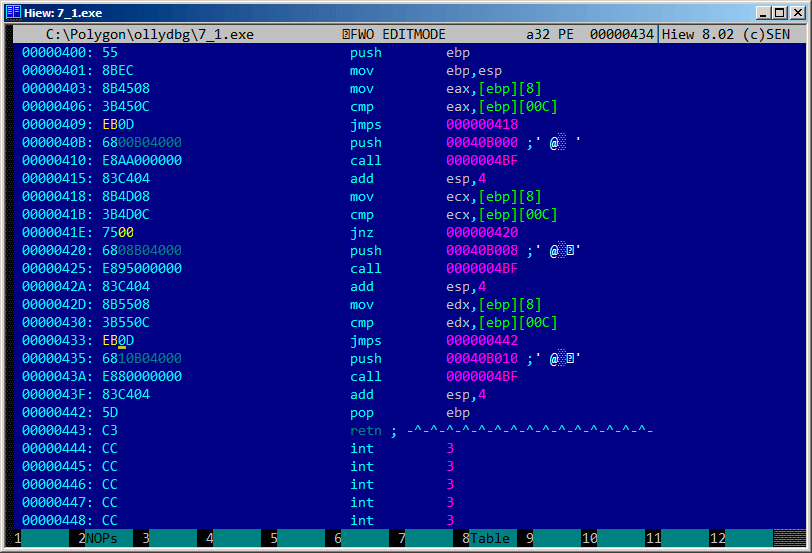
\includegraphics[scale=\FigScale]{patterns/07_jcc/simple/hiew_unsigned2.png}
\caption{Hiew: let's modify the \TT{f\_unsigned()} function}
\label{fig:jcc_hiew_2}
\end{figure}

If we miss to change any of these jumps, then several \printf calls may execute, while we want to execute only one.

\subsubsectionold{\NonOptimizing GCC}

\myindex{puts() instead of printf()}
\NonOptimizing GCC 4.4.1 
produces almost the same code, but with \puts~(\myref{puts}) instead of \printf.

\subsubsectionold{\Optimizing GCC}

An observant reader may ask, why execute \CMP several times, 
if the flags has the same values after each execution?

Perhaps optimizing MSVC can not do this, but optimizing GCC 4.8.1 can go deeper:

\lstinputlisting[caption=GCC 4.8.1 f\_signed()]{patterns/07_jcc/simple/GCC_O3_signed.asm}

% should be here instead of 'switch' section?
We also see \TT{JMP puts} here instead of \TT{CALL puts / RETN}.

This kind of trick will have explained later: \myref{JMP_instead_of_RET}.

This type of x86 code 
is somewhat rare.
MSVC 2012 as it seems, can't generate such code.
On the other hand, assembly language programmers are fully aware of the fact that \TT{Jcc} 
instructions can be stacked.

So if you see such stacking somewhere, it is highly probable that the code was hand-written.

The \TT{f\_unsigned()} function is not that 
\ae{}sthetically short:

\lstinputlisting[caption=GCC 4.8.1 f\_unsigned()]{patterns/07_jcc/simple/GCC_O3_unsigned_EN.asm}

Nevertheless, there are two \TT{CMP} instructions instead of three.

So optimization algorithms of GCC 4.8.1 are probably not perfect yet. 
